\documentclass[varwidth]{article}
\usepackage[utf8]{inputenc}
\usepackage{tikz,tcolorbox, tikz-cd, float}
\usetikzlibrary{quotes,angles, positioning}
\usepackage{amsfonts, amsmath, amssymb, fixmath}
\usepackage[table]{xcolor} 
\usepackage{standalone}
\title{RL3 - Planning By Dynamic Programming}
\author{sumit singh}
\date{\today}

\begin{document}

\maketitle

\section{Introduction}
\subsection{Dynamic Programming}
What is Dynamic Programming? \\
\begin{itemize}
    \item Dynamic: sequential or temporal component to the problem 
    \item Programming: optimising a "program", i.e. a policy. c.f. Linear Programming 
    \item A method for solving complex problems
    \item By breaking them down into subproblems and solve the subproblems
\end{itemize}
\subsubsection{Requirements for Dynamic Programming}
Dynamic Programming is a very general solution method for problems which have two properties:
\begin{itemize}
    \item Optimal substructure
    \begin{itemize}
        \item \textit{Principle of optimality} applies
        \item Optimal solution can be decomposed into sub problems
    \end{itemize}
    \item Overlapping sub-problems
    \begin{itemize}
        \item Sub problems recur many times
        \item Solutions can be cached and reused
    \end{itemize}
    \item Markov Decision Process satisfies both properties.
    \begin{itemize}
        \item Bellman equation gives recursive decomposition
        \item Value function stores and reuses solutions
    \end{itemize}
\end{itemize}
\subsubsection{Planning by Dynamic Programming}
\begin{itemize}
    \item Dynamic Programming assumes full knowledge of the MDP
    \item It is used for planning in an MDP
    \item For prediction:
    \begin{itemize}
        \item Input: MDP $(S,A,P,R,\gamma)$ and policy $\pi$
        \item or: MRP $(S,P^\pi,R^\pi,\gamma)$
        \item Output: value function $v_\pi$
    \end{itemize}
    \item Or for control: 
    \begin{itemize}
        \item Input: MDP $(S,A, P,R,\gamma)$
        \item Output: optimal value function $v_*$
        \item and: optimal policy $\pi_*$
    \end{itemize}
\end{itemize}
\subsubsection{Other Applications of Dynamic Programming}
\begin{itemize}    
    \item Dynamic Programming is used to solve many other problems, e.g.
    \begin{itemize}
        \item Scheduling algorithms
        \item String algorithms (e.g. sequence alignment)
        \item Graph algorithms (e.g. shortest path algorithms)
        \item Graphical models (e.g. Viterbi algorithm)
        \item Bioinformatics (e.g. lattice models)
    \end{itemize}
\end{itemize}
%*************************************************************************************************************
\section{Policy Evaluation}
\subsection{Iterative Policy Evaluation}


\begin{itemize}
    \item Problem: evaluate a given policy $\pi$
    \item Solution: iterative application of Bellman expectation backup
    \item $v_1 \rightarrow v_2 \rightarrow \cdots \rightarrow v_\pi  $
    \item Using \textit{synchronous} backups
    \begin{itemize}
        \item At each iteration $k+1$
        \item For all states $s\in S$
        \item Update $v_{k+1}(s) $ from $v_k(s')$
        \item where $s'$ is a successor state of $s$
    \end{itemize}
    \item We will discuss \textit{asynchronous} backup later
    \item Convergence to $v_\pi$ will pe proven at the end of the lecture
\end{itemize}
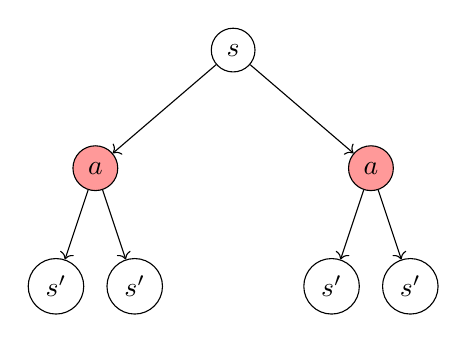
\begin{tikzpicture}[
    level distance=1.5cm,
    level 1/.style={sibling distance=3.5cm},
    level 2/.style={sibling distance=1cm}, ->]
    \tikzstyle{every node}=[circle,draw]
                
    \node (Root)  {$s$}
    child {
        node[fill=red!40] {$a$} 
        child { node {$s'$} }
        child { node {$s'$} }
    }
    child {
        node[fill=red!40] {$a$}
        child { node {$s'$} }
        child { node {$s'$} }
    }
    ;
\end{tikzpicture}
$$ v_{k+1}(s)  = \sum_{a \in A} \pi (a|s) \bigg( R_s^a + \gamma \sum_{s' \in S} P_{SS'}^a v_k(s')
\bigg)  $$
$$ \mathbold{v}^{k+1} = \mathbold{R^\pi}  + \gamma \mathbold{P^\pi v}^k $$
\newpage
\subsection{Evaluating a Random Policy in the Small Gridworld}
\begin{figure}[H]
  \centering
  \includestandalone[width=0.3\textwidth]{RL3_gridworld1}%     without .tex extension
  % or use \input{mytikz}
  \caption{Small Gridworld}
  \label{fig:tikz:my}
\end{figure}

\begin{itemize}
    \item Undiscounted episodic MDP $(\gamma = 1)$
    \item Non-terminal states $1, \cdots , 14$
    \item One terminal state (shown twice as shaded squares)
    \item Actions leading out of the grid leave state unchanged
    \item Reward is -1 until the terminal state is reached
    \item Agent follows uniform random policy
    $$\pi(n|.) = \pi(e|.) = \pi(s|.) = \pi(w|.) = 0.25 $$
\end{itemize}
\begin{center}
\begin{figure}[H]
  \centering
  \includestandalone[width=\textwidth]{RL3_gridworld2}%     without .tex extension
  % or use \input{mytikz}
  \caption{Iteration Policy Evaluation in Small Gridworld}
  \label{fig:tikz:my}
\end{figure}
\end{center}

\begin{figure}[H]
  \centering
  \includestandalone[width=\textwidth]{RL3_gridworld3}%     without .tex extension
  % or use \input{mytikz}
  \caption{Iteration Policy Evaluation in Small Gridworld (Optimal Policy)}
  \label{fig:tikz:my}
\end{figure}

%*************************************************************************************************************
\section{Policy Iteration}
\begin{figure}[H]
  \centering
  \includestandalone[width=\textwidth]{RL3_Policy_Iteration2}%     without .tex extension
  % or use \input{mytikz}
  \caption{Iteration Policy Evaluation in Small Gridworld (Optimal Policy)}
  \label{fig:tikz:my}
\end{figure}
\begin{itemize}
    \item \textcolor{blue}{Policy Evaluation} Estimate $v_\pi$ Iterative policy evaluation 
    \item \textcolor{blue}{Policy Improvement} Generate $\pi' \geq \pi $ Greedy policy improvement.
\end{itemize}
\subsection{How to improve a policy?}
\begin{itemize}
    \item Given a policy $\pi$
    \begin{itemize}
        \item \textcolor{red}{Evaluate} the policy $\pi$
        $$ v_\pi(s) = \mathbb{E}[R_{t+1} + \gamma R_{t+2} + \cdots | S_t = s] $$
        \item \textcolor{red}{Improve} the policy by acting greedily with respect to $v_\pi$
        $$\pi' = greedy(v_\pi)$$
    \end{itemize}
    \item In Small Gridworld improved policy was optimal, $\pi' = \pi^*$
    \item In general, need more iterations of improvement/evaluation
    \item But this process of \textcolor{red}{policy iteration} always converges to $\pi^*$
\end{itemize}
\subsection{Policy Improvement}
\begin{itemize}
    \item Consider a Deterministic Policy $ a = \pi(s) $
    \item We can \textit{improve} the policy by acting greedily
    $$ \pi'(s) = \underset{a\in A}{\mathrm{argmax}}\, q_{\pi}(s,a) $$
    \item This improves the value from any state $s$ over one step,
    $$ q_{\pi}(s,\pi'(s)) = \underset{a \in A}{\mathrm{max}}\, q_{\pi}(s,a) \ge q_{\pi}(s,\pi(s)) = v_{\pi}(s)   $$
   

    \item It therefore improves the value function,
    $$v_{\pi'}(s) \ge v_{\pi}(s)$$

    \begin{align*}
        v_{\pi}(s) &\leq q_{\pi}(s,\pi'(s)) = \mathbb{E} _{\pi'}[R_{t+1} + \gamma v_\pi (S_{t+1}) |S_t = s]\\
        &\leq \mathbb{E}_{\pi'} [R_{t+1} + \gamma q_\pi(S_{t+1}, \pi'(S_{t+1})) | S_t = s] \\
        &\leq \mathbb{E}_{\pi'} [R_{t+1} + \gamma R_{t+2} + \gamma^2 q_\pi (S_{t+2}, \pi'(S_{t+2})) | S_t = s ] \\
        &\leq \mathbb{E}_{\pi'} [R_{t+1} + \gamma R_{t+2} + \cdots | S_t = s ] = v_{\pi'}(s)
    \end{align*}
\end{itemize}

\begin{itemize}
    \item If improvement stop,
    $$ q_\pi(s,\pi'(s)) =  \underset{a \in A}{\mathrm{max}}\, q_\pi(s,a) = q_\pi(s, \pi(s)) = v_\pi(s) $$
    \item Then the Bellman optimality equation has been satisfied
    $$ v_\pi(s) = \underset{a \in A}{\mathrm{max}}\, q_\pi(s,a) $$
    \item Therefore $v_\pi(s)  = v_*(s) \forall s \in S$
    \item so $\pi$ is an optimal policy
\end{itemize}



%*************************************************************************************************************
\section{Value Iteration}
%*************************************************************************************************************
\section{Extensions to Dynamic Programming}
%*************************************************************************************************************
\section{Contraction Mapping}

%*************************************************************************************************************
\section{References}
\end{document}